%!TEX program = xelatex

% \documentclass[printbox,marginline,noindent]{BHCexam1}
\documentclass{BHCexam1}
\usepackage{gensymb}
\usepackage{mathrsfs}
\usepackage{tikz,pgfplots,float} %绘图
\usepackage{tkz-euclide}
\usepackage{wrapfig}
\usepackage[english]{babel}
\usepackage{caption}
\usepackage{CJK}
\usepackage{enumitem}
\usetikzlibrary{calc,quotes,angles,babel,intersections,arrows,automata,positioning}

\pgfplotsset{compat=1.15}
\tikzset{ 
  right angle quadrant/.code={ 
   \pgfmathsetmacro\quadranta{{1,1,-1,-1}[#1-1]} % Arrays for selecting quadrant 
   \pgfmathsetmacro\quadrantb{{1,-1,-1,1}[#1-1]}}, 
  right angle quadrant=1, % Make sure it is set, even if not called explicitly 
  right angle length/.code={\def\rightanglelength{#1}}, % Length of symbol 
  right angle length=2ex, % Make sure it is set... 
  right angle symbol/.style n args={3}{ 
   insert path={ 
   let \p0 = ( $(#1)!(#3)!(#2)$ ) in % Intersection 
    let \p1 = ( $(\p0)!\quadranta*\rightanglelength!(#3)$ ), % Point on base line 
    \p2 = ( $(\p0)!\quadrantb*\rightanglelength!(#2)$ ) in % Point on perpendicular line 
    let \p3 = ( $(\p1)+(\p2)-(\p0)$ ) in % Corner point of symbol 
   (\p1) -- (\p3) -- (\p2) 
   } 
  } 
}
\begin{document}
\maketitle
\begin{questions}

\question%% Question ID: 14c9c266-0c20-11e9-8b4a-520090400c01
如图,直线~$AB,CD$~相交于点~$O$,已知$\angle AOD=130\degree$,$\angle AOC:\angle EOC=5:4$,求$\angle BOE$的大小.

\hfill
\begin{tikzpicture}[scale=0.8]
\coordinate[label=below left:$O$] (O) at (0,0);
\coordinate[label=below:$A$] (A) at (-3,0);
\coordinate[label=below:$B$] (B) at (3,0);
\coordinate[label=above:$E$] (E) at (0,3);
\draw (A) -- (B);
\draw (O) -- (E);
\begin{scope}[rotate=-50,shift={(-1,0)}]
\coordinate[label=above left:$C$] (C) at (-3,0);
\coordinate[label=above right:$D$] (D) at (3,0);
\draw (C) -- (D);
\end{scope}
\end{tikzpicture}


%%% -------- Anchor End ---------- %%%
\question%% Question ID: 6f894712-0c20-11e9-8b4a-520090400c01
如下图,已知在直角~$\triangle ABC$~中,~$\angle C=90\degree$,~$AC=7$,$BC=5$,
% \stk{}

\begin{enumerate}[label={(\arabic*)}]
\item 点到的距离为\stk 。
\item 在图中作出点到的距离。
\end{enumerate}
% \twoch{a}{b}{c}{d}
\hfill
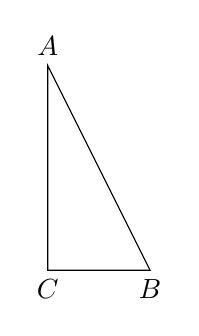
\begin{tikzpicture}[scale=1.3]
\coordinate [label=below:$C$] (C) at (0,0);
\coordinate [label=below:$B$] (B) at (1,0);
\coordinate [label=above:$A$] (A) at (0,2);
\draw (C) -- (B) -- (A) -- cycle;
\end{tikzpicture}

%%% -------- Anchor End ---------- %%%
\question%% Question ID: eec18296-0c17-11e9-8a2e-520090400c01
已知长方形$ABCO$,~$O$为坐标原点,点$B$的坐标为$(8,6)$,~$A,C$分别在坐标轴上,$P$是线段$BC$上动点,设$PC=m$,已知点$D$在第一象限且是直线$y=2x+6$上的一点,若$\triangle APD$是等腰直角三角形。
\begin{enumerate}[label={(\arabic*)}]
\item 求点$D$的坐标;
\item 直线$y=2x+6$向右平移6个单位后,在该直线上,是否存在点$D$,使$\triangle APD$是等腰三角形?若存在,请求出这些点的坐标;若不存在,请说明理由。
\end{enumerate}

% \hskip 50pt
\hfill
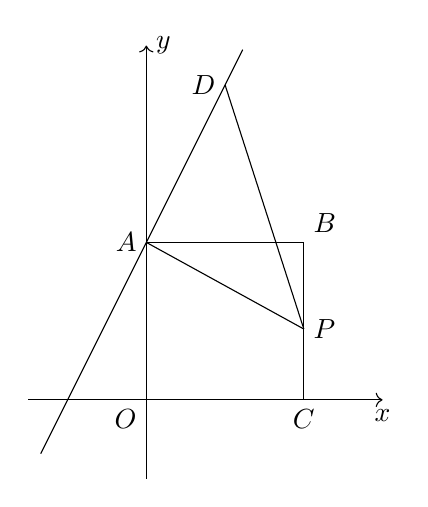
\begin{tikzpicture}[dot/.style={circle,inner sep=1pt,fill,label={#1},name=#1},
 extended line/.style={shorten >=-#1,shorten <=-#1},
 extended line/.default=1cm] %[scale=0.6]
\coordinate [label= below left:$O$] (O) at (0,0);
\coordinate [label= below:$C$] (C) at (2,0);
\coordinate [label= left:$A$] (A) at (0,2);
\coordinate [label= above right:$B$] (B) at (2,2);
\coordinate [label= left:$D$] (D) at (1,4);
\coordinate [label= right:$P$] (P) at($(B)!0.55!(C)$);
\draw [extended line,shorten >=-0.5cm,shorten <=-3cm] (A) -- (D);
\draw (A) -- (B);
\draw (B) -- (C);
\draw (D) -- (P);
\draw (A) -- (P);
\draw [->] (O)+(-1.5,0) -- (3,0) node [below]{$x$};
\draw [->] (O)+(0,-1) -- (0,4.5) node [right]{$y$};
\end{tikzpicture}

%%% -------- Anchor End ---------- %%%
\question%% Question ID: ba3e123c-0c17-11e9-8a2e-520090400c01
如图,在$\triangle ABC$中,$\angle ACB=90\degree$,$\angle A=30 \degree,~D$是边$AC$上不与点$A$、$C$重合的任意一点,
$DE\bot AB$,垂足为点$E$,$M$是$BD$的中点.
% \stk{}

\begin{enumerate}[label={(\arabic*)}]
\item 求证:$CM=EM$~;
\item 如果~$BC=\sqrt{3}$,设~$AD=x,~CM=y$,求$y$与$x$的函数解析式,并写出定义域;
\item 当点$D$在线段$AC$上移动时,$\angle MCE$~的大小是否发生变化?若不变,求出~$\angle MCE$~的大小;如果发生变化,说明如何变化.
\end{enumerate}
% \twoch{a}{b}{c}{d}
\hfill
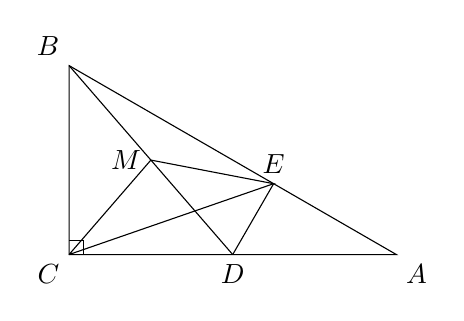
\begin{tikzpicture}[scale=0.6]
%\draw [help lines] (0,0) grid (7,4);
\coordinate[label=below left:$C$] (C) at (0,0);
\coordinate[label=above left:$B$] (B) at (0,4);
\coordinate[label=below right:$A$] (A) at ({4*sqrt(3)},0);
\draw [right angle symbol={B}{C}{A}]; 
\draw (A) -- (B) -- (C) -- cycle;
\coordinate[label=below:$D$] (D) at($(C)!0.5!(A)$);
\draw (B) -- (D);
\draw ( $(A)!(D)!(B)$ ) coordinate[label=above:$E$] (E) -- (D); 
\coordinate[label=left:$M$] (M) at($(B)!0.5!(D)$);
\draw (C) -- (M) -- (E) -- (C);
% \draw[blue,->] (C) -- ($(A)!(C)!(B)$);
\end{tikzpicture}

%%% -------- Anchor End ---------- %%%
\end{questions}
\end{document}